\chapter{User manual for working with the smart Inter Circuit Tests (ICT) analyzer tool}
This document describes the way of handling the tool for determining the test coverage of different \ac{ODB}++ related projects.
\section{Overview}

\begin{center}
	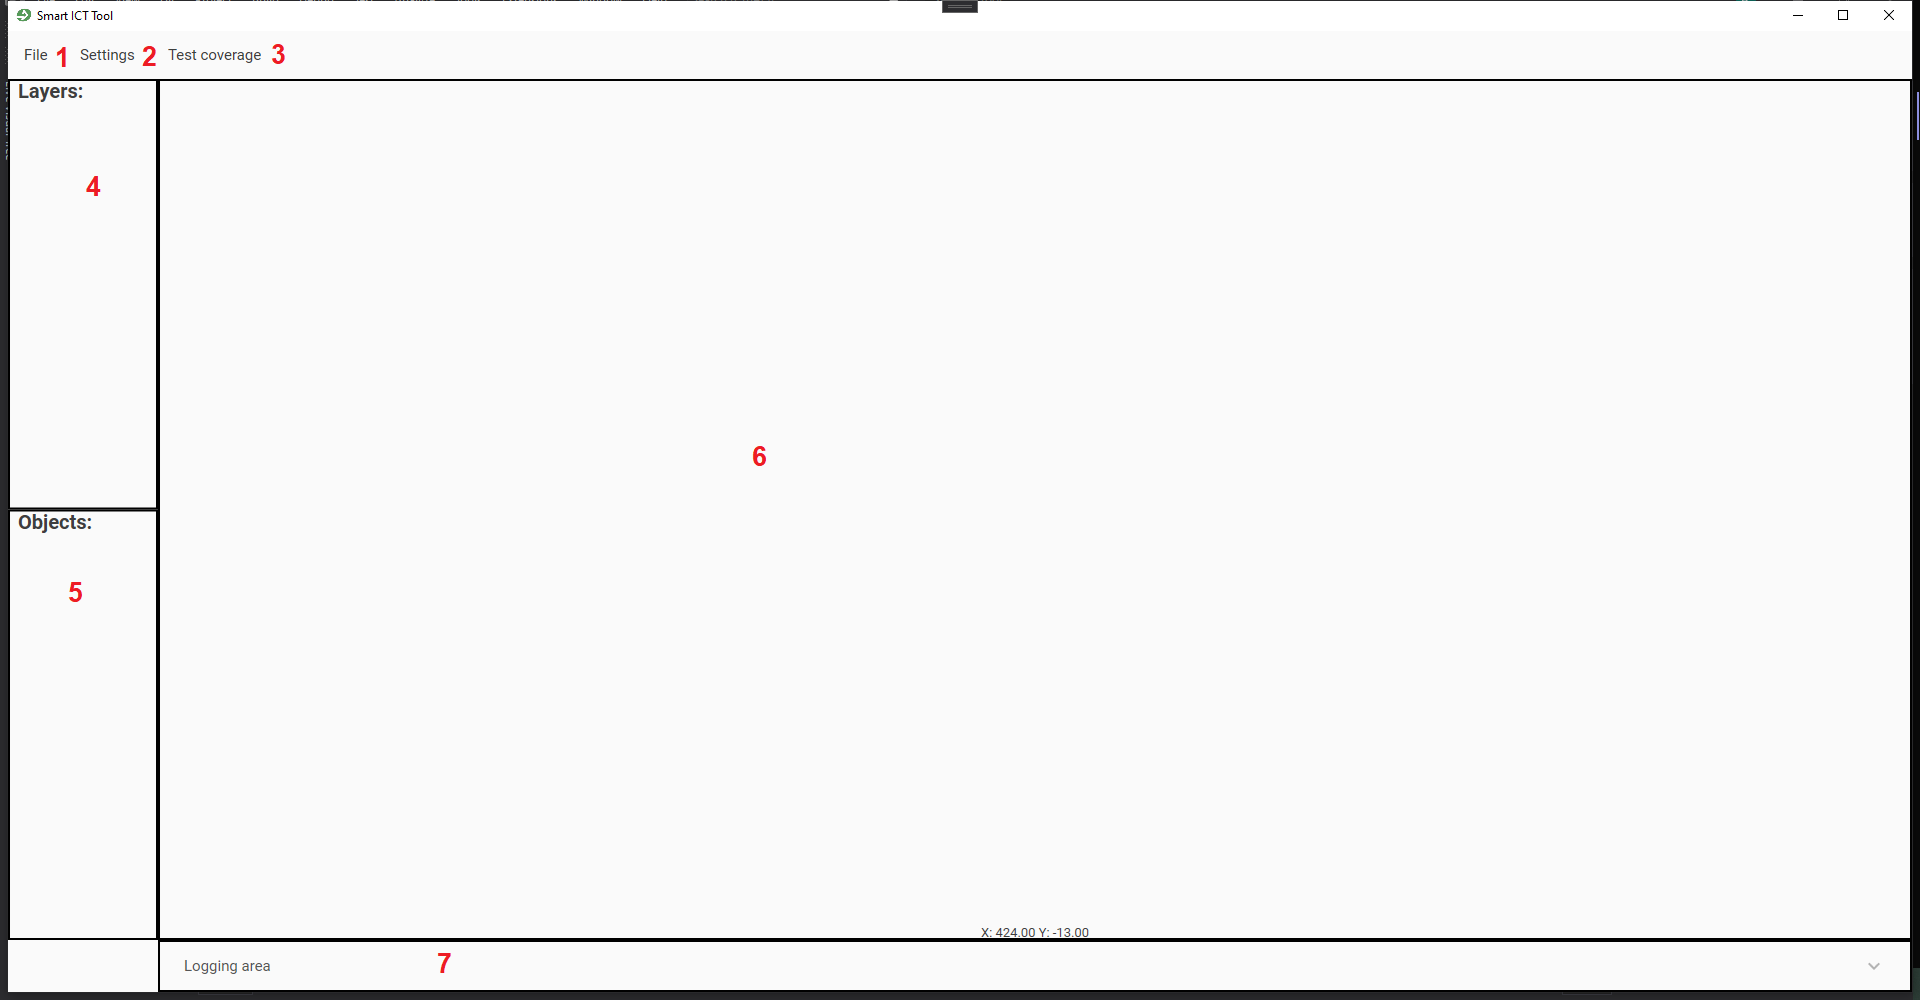
\includegraphics[width=1.00\textwidth]{figures/attachments/overview.png}
	\begin{figure}[!h]
	\caption{Tool overview}
	\label{fig:Tooloverview}
	\end{figure}
\end{center}

As shown in \ref{fig:Tooloverview} the tool itself consists of seven different areas of interest:
\begin{enumerate}
	\item File menu group - performing actions regarding the opening of project files, ...
	\item Settings - selection of settings, importing and exporting them
	\item Test coverage - all test coverage related actions
	\item Layers - the layers overview
	\item Objects - the test coverage objects list
	\item the rendered component view
	\item The logging area
\end{enumerate}

\section{Settings}

\begin{center}
	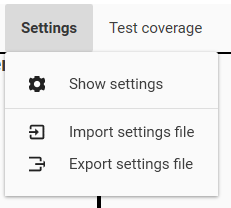
\includegraphics[scale=0.60]{figures/attachments/settingsOverview.png}
	\begin{figure}[!h]
	\caption{Settings overview}
	\label{fig:Settingsoverview}
	\end{figure}
\end{center}

As shown in \ref{fig:Settingsoverview} there are the following three menu items available:
\begin{enumerate}
	\item Show settings - opens the settings page for all settings
	\item Import settings file - a file chooser will pop up for selecting a settings database file to be imported
	\item Export settings file - a file chooser will pop up for selecting the target file where the settings database should be exported to
\end{enumerate}

\subsection{Show settings}
After clicking on the menu item All settings a new window will be shown containing all setting pages.
\subsubsection{PCB Investigator \ac{API} settings}

\begin{center}
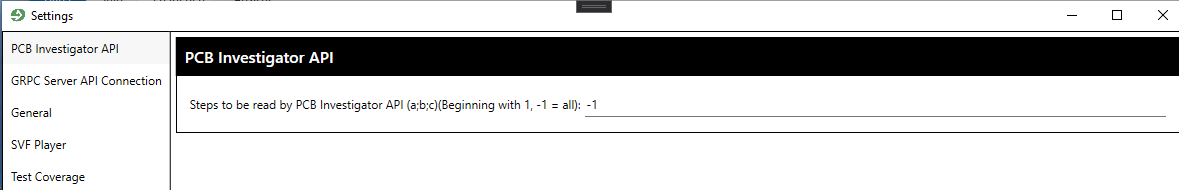
\includegraphics[width=1.00\textwidth]{figures/attachments/pcbInvestigatorSettings.png}
	\begin{figure}[!h]
	\caption{PCB Investigator \ac{API} settings}
	\label{fig:pcbInvestigatorSettings}
	\end{figure}
\end{center}

As shown in \ref{fig:pcbInvestigatorSettings} there is the possibility of changing the steps which should be considered for read out from the \ac{API}. -1 means all steps should be read out. Other values could be defined semicolon separated

\subsubsection{GRPC server \ac{API} connection settings}

\begin{center}
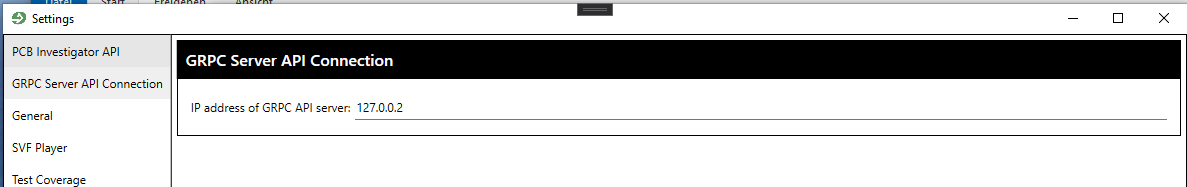
\includegraphics[width=1.00\textwidth]{figures/attachments/grpcServerSettings.png}
	\begin{figure}[!h]
	\caption{\ac{GRPC} server \ac{API} connection settings}
	\label{fig:grpcServerSettings}
	\end{figure}
\end{center}

As shown in \ref{fig:grpcServerSettings} there is the possibilty of changing the ip address of the \ac{GRPC} server to connect to

\subsubsection{General settings}

\begin{center}
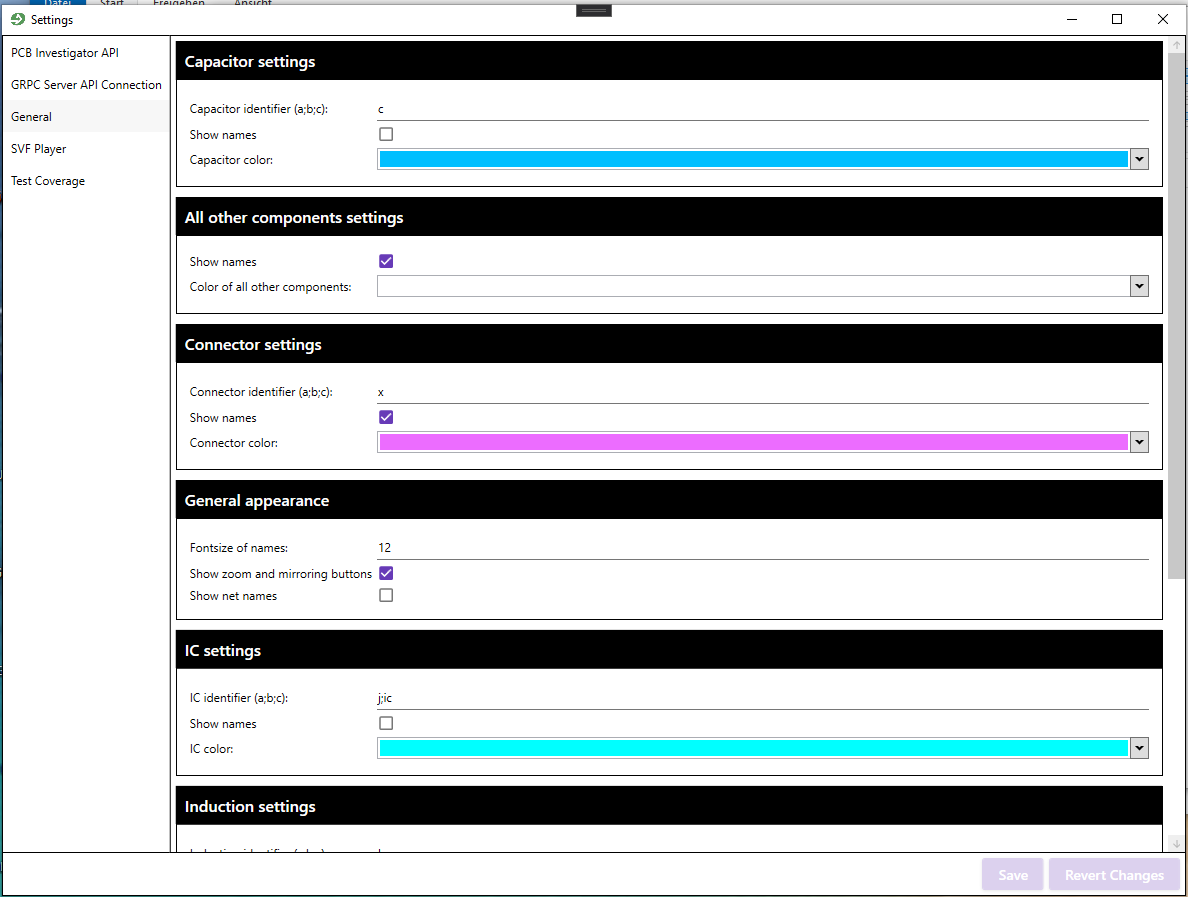
\includegraphics[width=1.00\textwidth]{figures/attachments/generalSettings1.png}
	\begin{figure}[!h]
	\caption{General settings 1}
	\label{fig:generalSettings1}
	\end{figure}
\end{center}

Within the first part of the general settings (\ref{fig:generalSettings1}) there are the following settings available (identifier, show names and the color):
\begin{itemize}
	\item Capacitor
	\item Other components
	\item Connector
	\item \ac{IC}
\end{itemize}
Fruthermore there are the following settings available:
\begin{itemize}
	\item General appearance
	\begin{itemize}
		\item Fontsize of names
		\item Show zoom and mirroring buttons
		\item Show net names
	\end{itemize}
\end{itemize}

\begin{center}
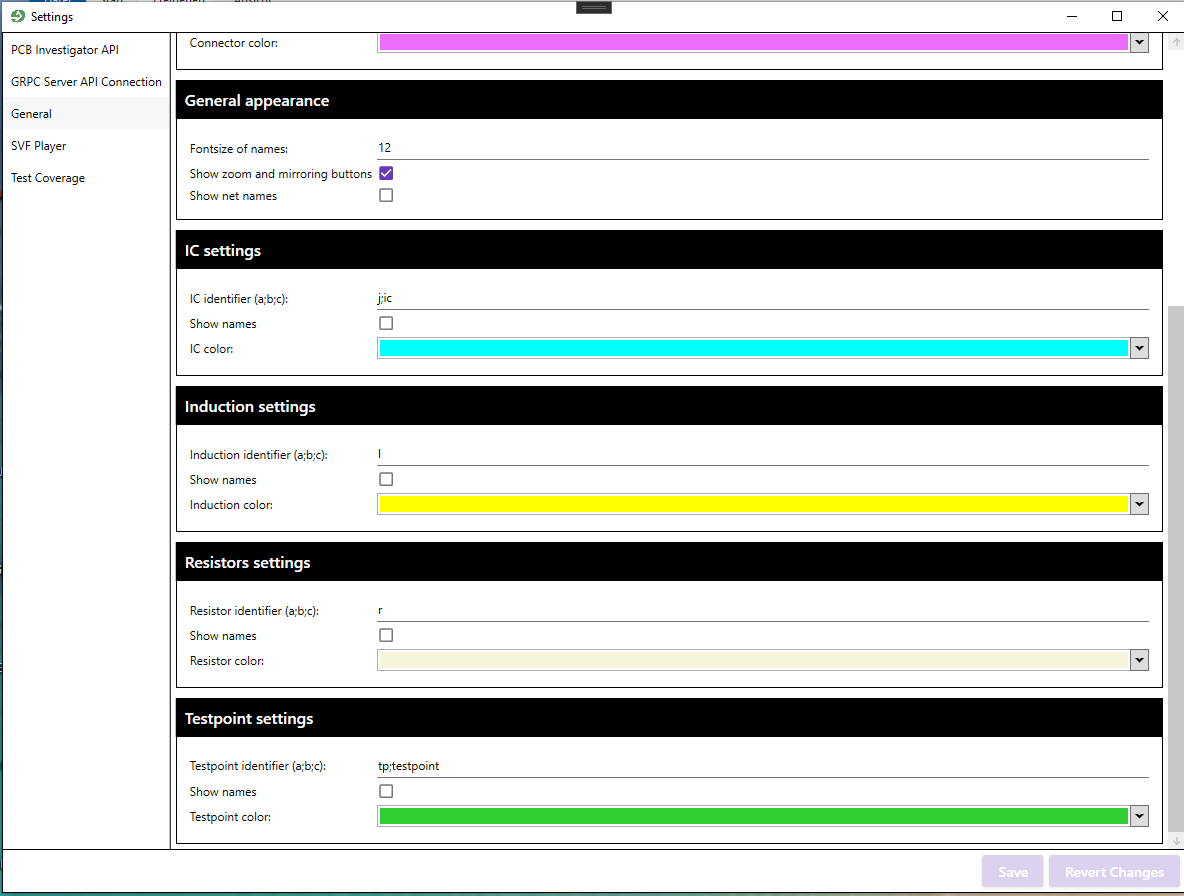
\includegraphics[width=1.00\textwidth]{figures/attachments/generalSettings2.png}
	\begin{figure}[!h]
	\caption{General settings 2}
	\label{fig:generalSettings2}
	\end{figure}
\end{center}

Within the second part of the general settings (\ref{fig:generalSettings2}) there are the following settings available (identifier, show names and the color):
\begin{itemize}
	\item Inductor
	\item Resistor
	\item Testpoint
\end{itemize}

\subsubsection{SVF Player settings}

\begin{center}
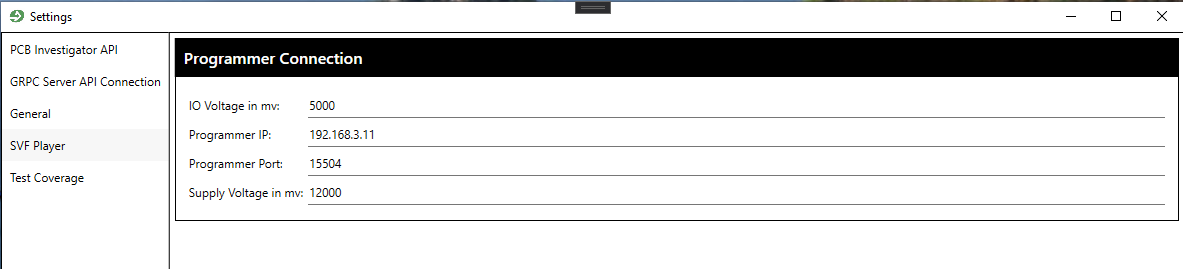
\includegraphics[width=1.00\textwidth]{figures/attachments/svfPlayerSettings.png}
	\begin{figure}[!h]
	\caption{\ac{SVF} Player settings}
	\label{fig:svfPlayerSettings}
	\end{figure}
\end{center}

As shown in \ref{fig:svfPlayerSettings} there are the following settings available:
\begin{itemize}
	\item IO Voltage in mv
	\item Programmer IP
	\item Programmer Port
	\item Supply Voltage in mv
\end{itemize}

\subsubsection{Test Coverage settings}

\begin{center}
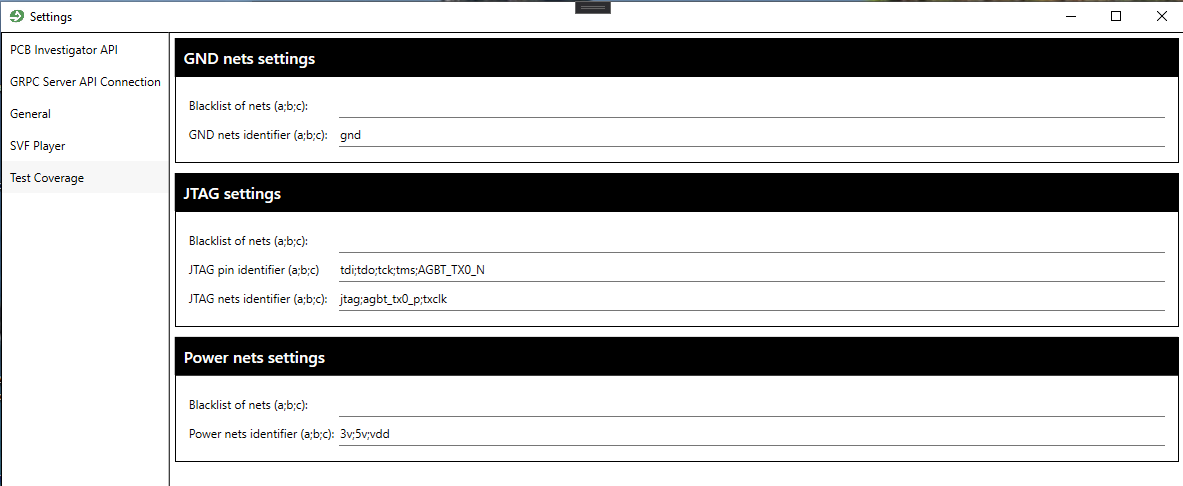
\includegraphics[width=1.00\textwidth]{figures/attachments/testCoverageSettings.png}
	\begin{figure}[!h]
	\caption{Test Coverage settings}
	\label{fig:testCoverageSettings}
	\end{figure}
\end{center}

As shown in \ref{fig:testCoverageSettings} there are the following settings available (blacklist of nets and net identifier):
\begin{itemize}
	\item Ground
	\item \ac{JTAG}
	\item Power
\end{itemize}
Further more there is the possibility of defining the \ac{JTAG} pin identifier for making sure being able to use not just the default values \textbf{TMS, TDI, TDO, TCK}. That means in detail for correctly determining a \ac{JTAG} device there should be the following requirements accomplished:
\begin{enumerate}
	\item Set up the \textbf{\ac{IC} identifier} setting from general settings in that way that the \ac{JTAG} device is being recognized correctly as an \ac{IC} component
	\item Set up the \textbf{\ac{JTAG} nets identifier} from the test coverage settings in that way that the \ac{JTAG} device is correctly being recognized within a corresponding net
	\item Set up the \textbf{\ac{JTAG} pin identifier} setting from the test coverage settings in that way that the \ac{JTAG} device is correctly being recognized by its pins
\end{enumerate}

\subsection{Import / Export settings file}
By clicking on one of the menu items Settings -> Import settings file or Settings -> Export settings file afterward a new file selection dialog will be shown where to select the source / target file to be imported / exported. Further if the project file handling is enabled the settings file will automatically be stored within the project file and be loaded automatically on next opening of project file

\section{Project file}

\begin{center}
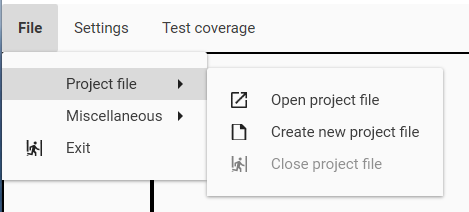
\includegraphics[scale=0.60]{figures/attachments/projectFile.png}
	\begin{figure}[!h]
	\caption{Project file handling}
	\label{fig:projectFile}
	\end{figure}
\end{center}

As shown in \ref{fig:projectFile} there is the possibility of choosing the following menu items within the File -> Project file group:
\begin{itemize}
	\item Open project file
	\item Create new project file
\end{itemize}

\section{Miscellaneous}

\begin{center}
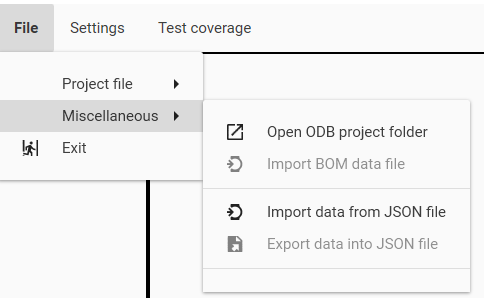
\includegraphics[scale=0.60]{figures/attachments/fileMisc.png}
	\begin{figure}[!h]
	\caption{Miscellaneous menu items}
	\label{fig:fileMisc}
	\end{figure}
\end{center}

As shown in \ref{fig:fileMisc} there are the following menu items available at File -> Miscellaneous:
\begin{itemize}
	\item Open \ac{ODB} project folder - after choosing that action a new dialog appears to select the folder which should be transferred to the \ac{GRPC} server as zipped content for read out by using the PCB-Investigator \ac{API}
	\item Import \ac{BOM} data file - After any project was successfully loaded then the import of a valid bill of materials file will be available. After choosing this a new window appears where to set up all relevant settings for import
	\item Import data from \ac{JSON} file - a new dialog appears where you are able to select any \ac{JSON} formatted file containing previously exported data of this application
	\item Export data into \ac{JSON} file - after any project was loaded successfully then this item will be accessible. After choosing it a new dialog appears where you could select the target for creation of a valid \ac{JSON} formatted file containing all data
\end{itemize}

\section{Creation of new project}
To create a new project just first click on File -> Project file -> Create new project file. After ward there will be a dialog shown for selecting the target file to be saved at:

\begin{center}
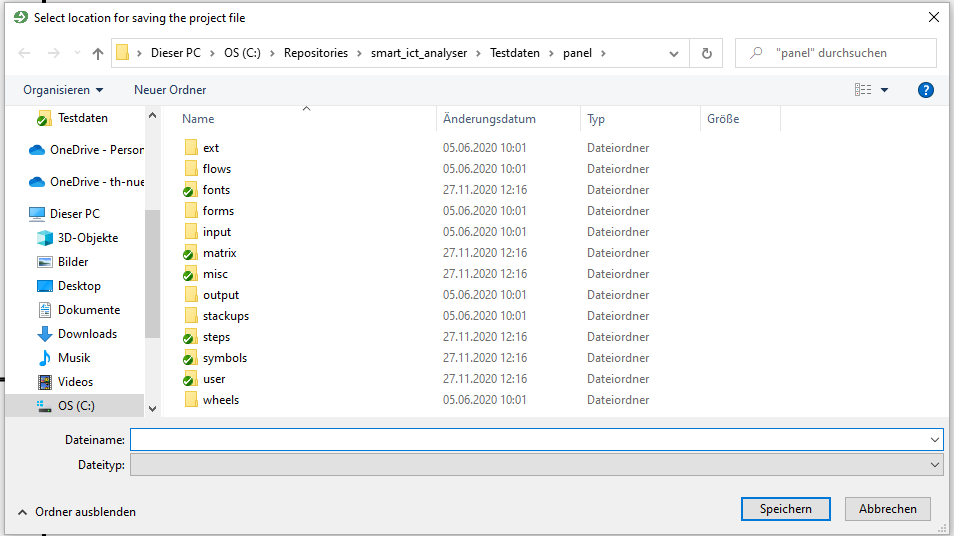
\includegraphics[scale=0.60]{figures/attachments/projectFileCreationDialog.png}
	\begin{figure}[!h]
	\caption{Project file creation dialog}
	\label{fig:projectFileCreationDialog}
	\end{figure}
\end{center}

After you confirmed your target within the dialog (\ref{fig:projectFileCreationDialog}) then you could proceed to open a new project. For that make sure to have a valid connection to the \ac{GRPC} server and click then File -> Miscellaneous -> Open \ac{ODB} project folder. After you chose a program during the communication and parsing from the \ac{GRPC} server there will be shown an animation:

\begin{center}
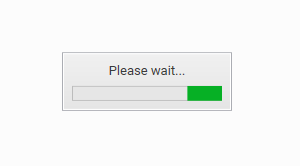
\includegraphics[scale=0.60]{figures/attachments/pleaseWait.png}
	\begin{figure}[!h]
	\caption{Please wait animation}
	\label{fig:pleaseWait}
	\end{figure}
\end{center}

After the process finished then if no values are defined for that components received a new dialog should be visible where to select the \ac{BOM} file for importing:

\begin{center}
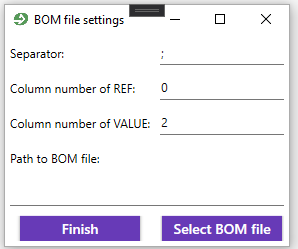
\includegraphics[scale=0.60]{figures/attachments/selectBom.png}
	\begin{figure}[!h]
	\caption{Select \ac{BOM} file dialog}
	\label{fig:selectBom}
	\end{figure}
\end{center}

After you set up the settings:
\begin{itemize}
	\item Separator
	\item Column number of REF
	\item Column number of VALUE
	\item Path to \ac{BOM} file - could be set by clicking on Select \ac{BOM} file where then a new dialog for selecting any file will be opened
\end{itemize}

within that dialog and selected a valid \ac{CSV} file to be imported then proceed by clicking on finish. \newline

After the process finished then on within the layers list there should be some layers available and the control buttons at the right bottom place will be visible:

\begin{center}
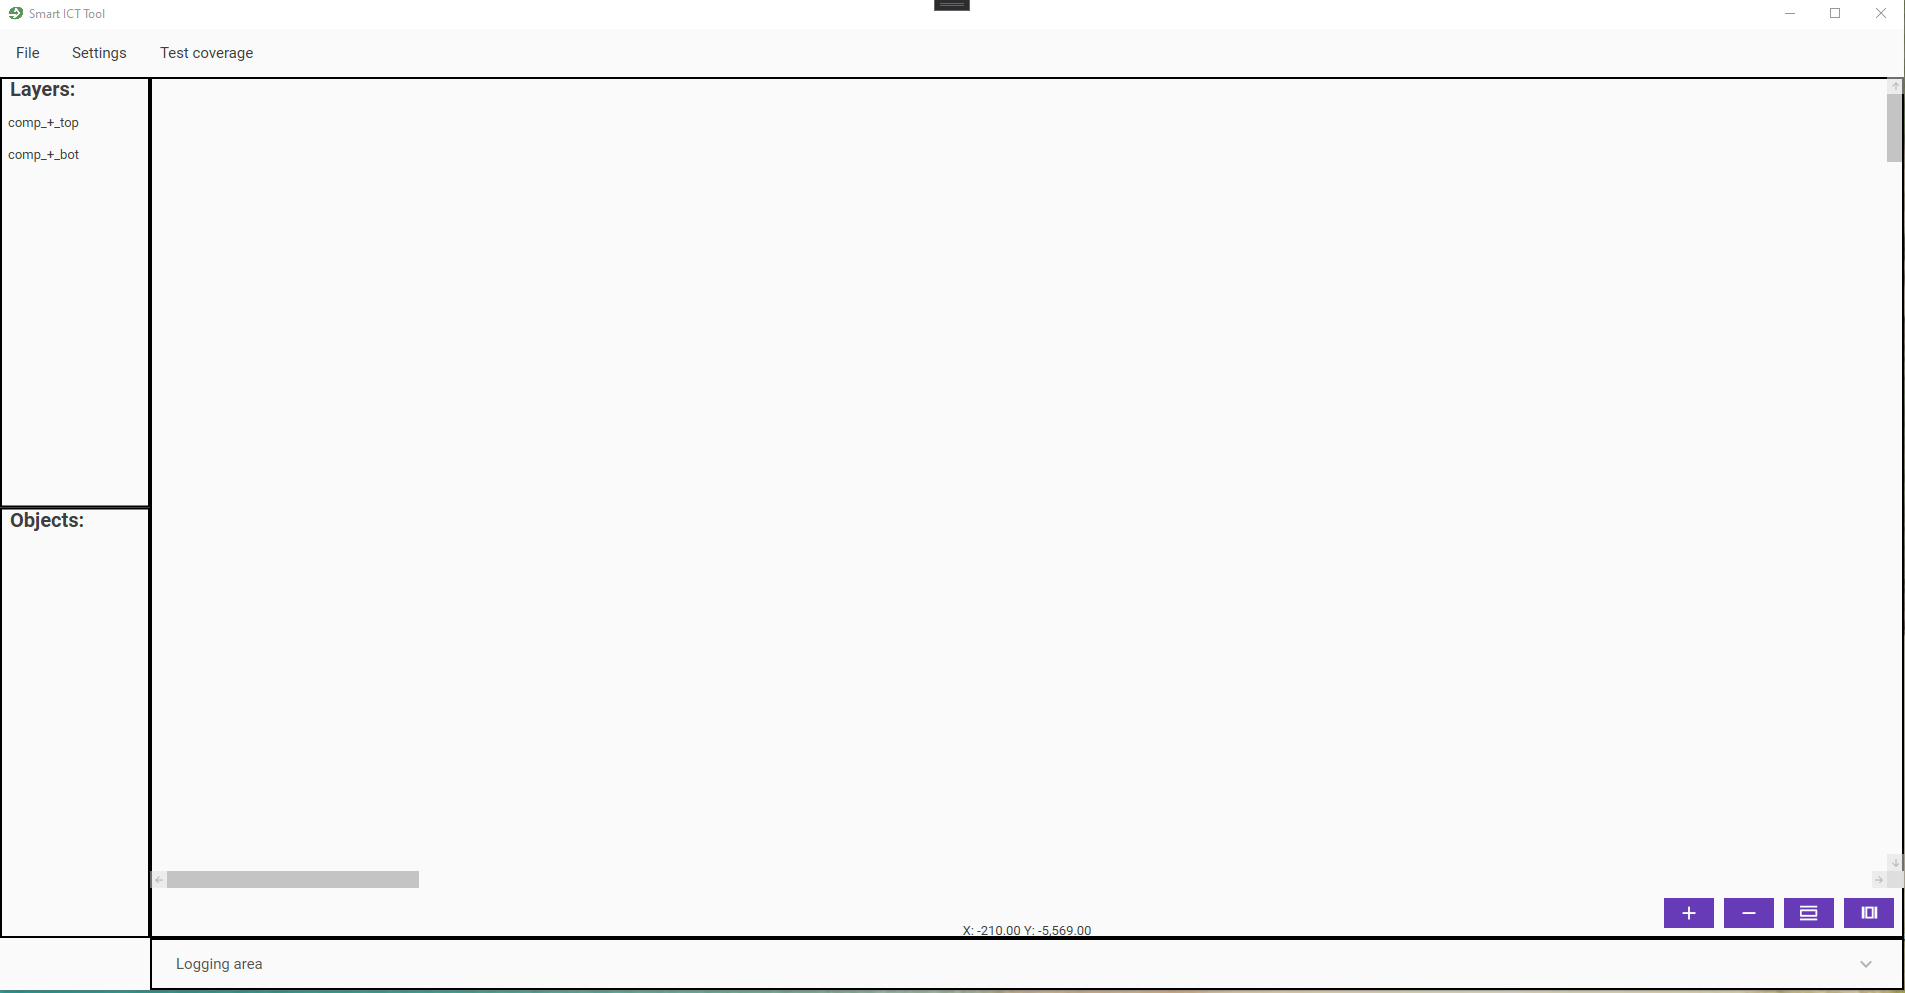
\includegraphics[width=1.00\textwidth]{figures/attachments/loadedProject.png}
	\begin{figure}[!h]
	\caption{Loaded project view}
	\label{fig:loadedProject}
	\end{figure}
\end{center}

After selecting for example the first layer then all components which are included within that layer should be rendered within the component view.

\begin{center}
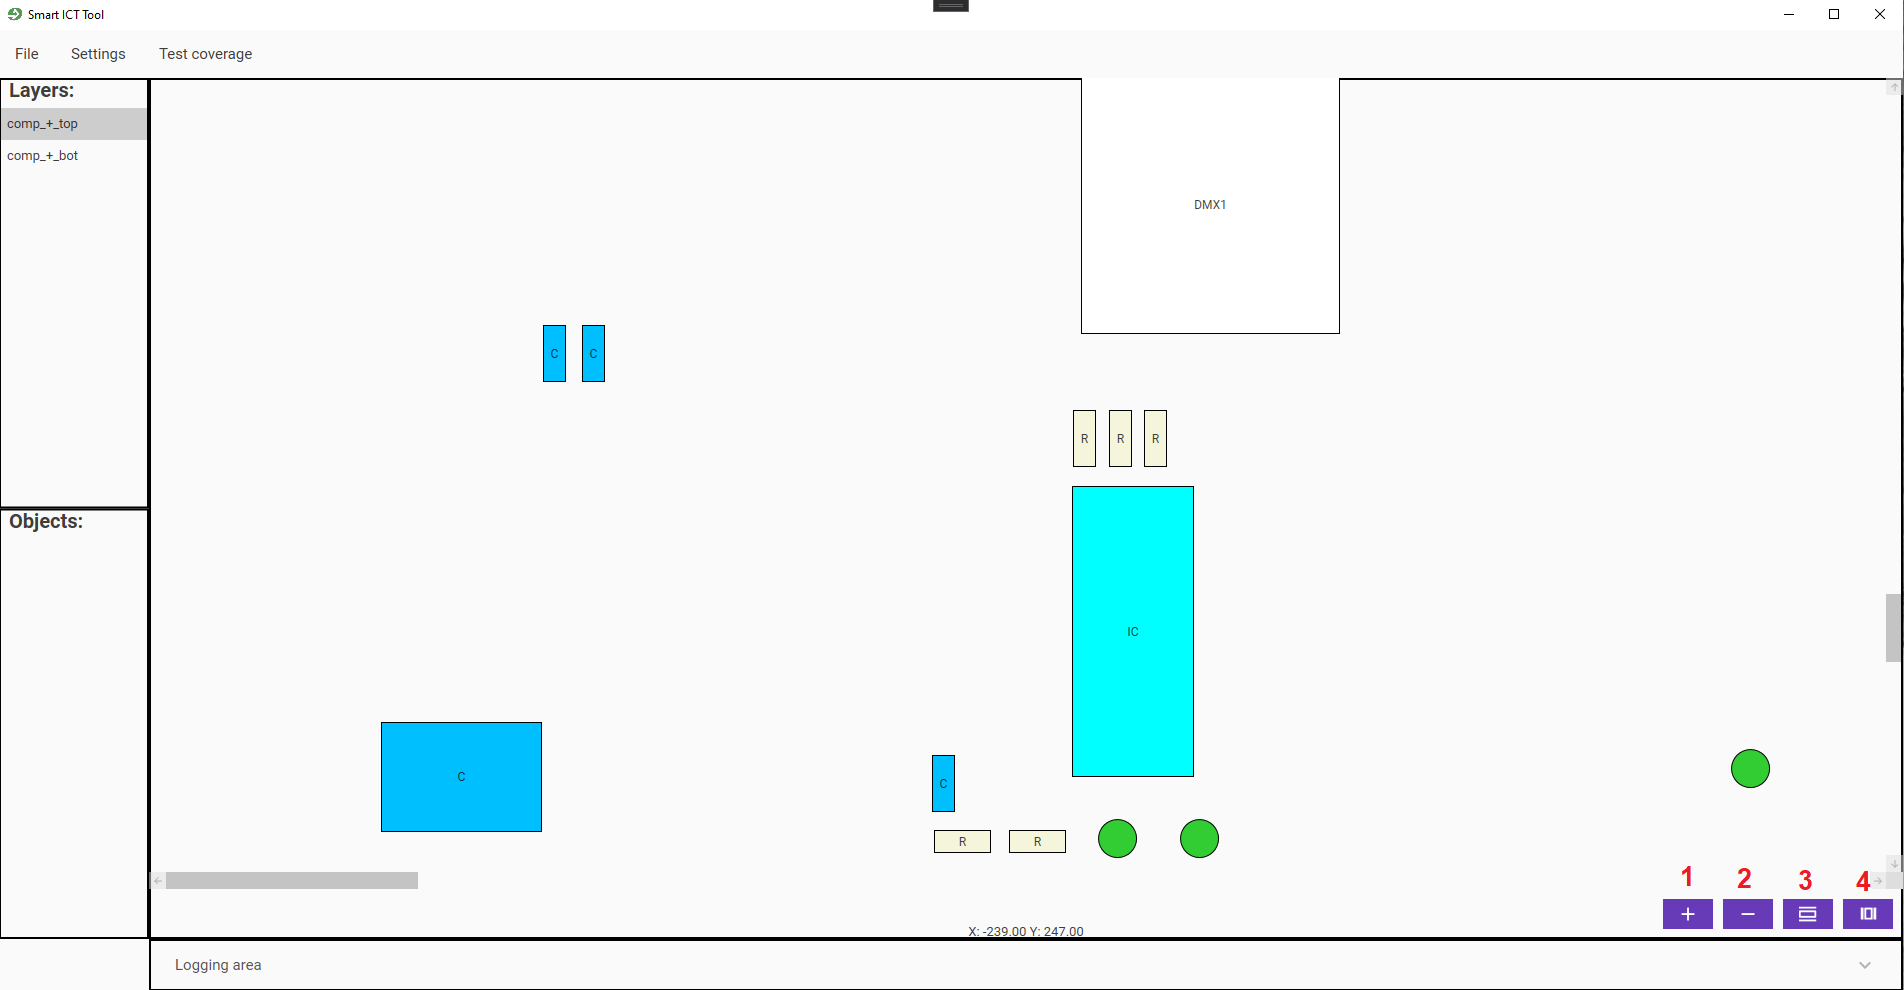
\includegraphics[width=1.00\textwidth]{figures/attachments/layerSelected.png}
	\begin{figure}[!h]
	\caption{Compontens view for selected layer}
	\label{fig:layerSelected}
	\end{figure}
\end{center}

As shown in \ref{fig:layerSelected} there is the possibility of scrolling with the mouse to move the whole view or just by clicking and dragging the whole content. Further there is the possibility of zooming in by pressing STRG and scrolling in or just by clicking on the zoom in button \textbf{1} and to zoom out by pressing STRG and scrolling out with the mouse or just by clicking the zoom out button \textbf{2}. Finally there is the possibility to mirror the whole view across the y axis \textbf{3} and the x axis \textbf{4}. Now to ensure not to have to use the \ac{GRPC} server again the next time you will open this project click File -> Miscellaneous -> Export data into \ac{JSON} file. After you chose it a new dialog will appear where you could type in just the name as the file itself will be stored within the project 
file as you are working within the project file mode. (Also all other project related data was automatically saved in the project file). Finally you should also 
export your current made settings by Settings -> Export settings file to make sure that the settings file is also included in the project file for later loading

\section{Working with the components view}
By right clicking on any object within the components view there will be a context menu visible:

\begin{center}
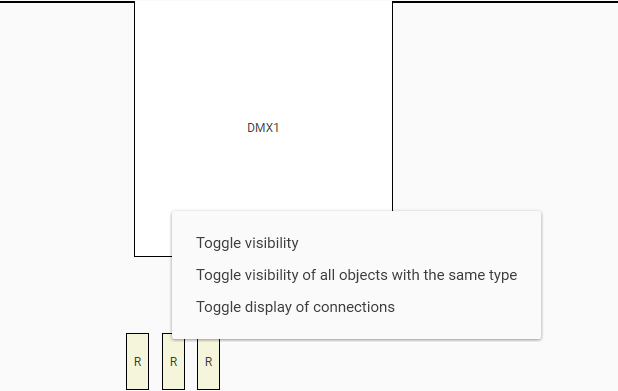
\includegraphics[scale=0.60]{figures/attachments/contextMenu.png}
	\begin{figure}[!h]
	\caption{Context menu of right click on component}
	\label{fig:contextMenu}
	\end{figure}
\end{center}

As shown at \ref{fig:contextMenu} you have the possibility of:
\begin{itemize}
	\item Toggle visibility - if clicked then the according components transparency will be set to high
	\item Toggle visibility of all objects with the same type - if clicked then all the according components which have the same type as the selected ones transparency will be set to high
	\item Toggle display of connections - if clicked then all connections of the component will be shown as plain lines
\end{itemize}

\subsection{Toggle visibility}

\begin{center}
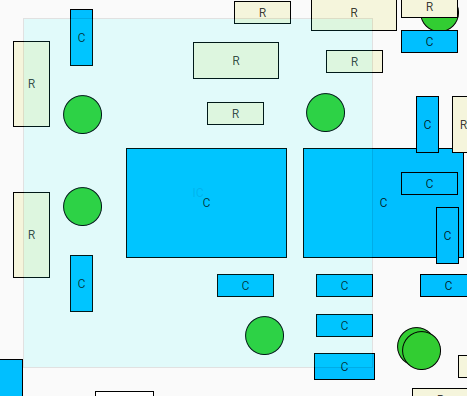
\includegraphics[scale=0.60]{figures/attachments/toggleVis.png}
	\begin{figure}[!h]
	\caption{Toggle visibility}
	\label{fig:toggleVis}
	\end{figure}
\end{center}

As shown in \ref{fig:toggleVis} after the visibility was toggled then the underlining objects could be determined

\subsection{Toggle visibility of all objects with the same type}

\begin{center}
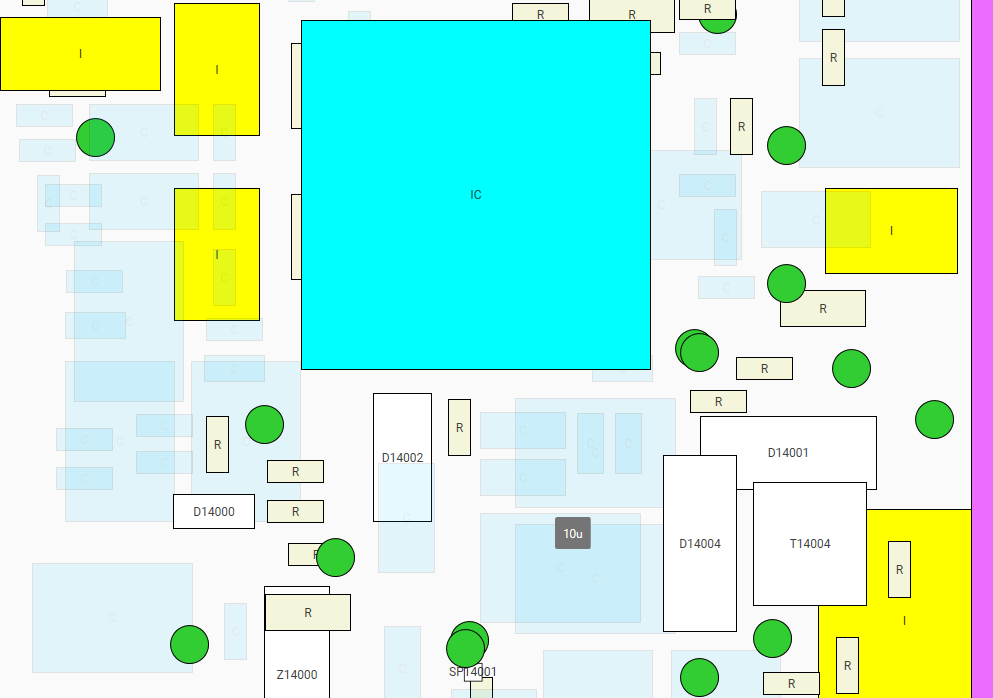
\includegraphics[scale=0.60]{figures/attachments/toggleVisAll.png}
	\begin{figure}[!h]
	\caption{Toggle visibility of all objects with the same type}
	\label{fig:toggleVisAll}
	\end{figure}
\end{center}

As shown in \ref{fig:toggleVis} after the visibility was toggled then the underlining objects of all toggled objects of the same type could be determined

\subsection{Toggle display of connections}

\begin{center}
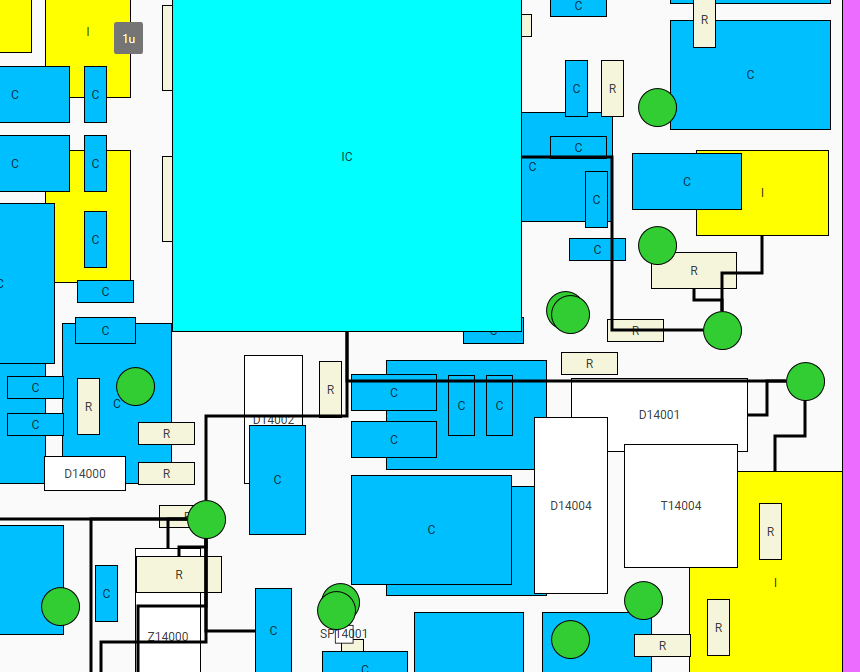
\includegraphics[scale=0.60]{figures/attachments/toggleConnection.png}
	\begin{figure}[!h]
	\caption{Toggle display of connections}
	\label{fig:toggleConnection}
	\end{figure}
\end{center}

As shown in \ref{fig:toggleConnection} after the connections were toggled then all lines will be drawn between the connecting objects.
Further there is the possibility to hover over any connection to see the following information:

\begin{center}
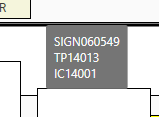
\includegraphics[scale=0.60]{figures/attachments/connectionLegend.png}
	\begin{figure}[!h]
	\caption{Legend of connection}
	\label{fig:connectionLegend}
	\end{figure}
\end{center}

As shown in \ref{fig:connectionLegend} there will be the following information available:

\begin{itemize}
	\item Net name
	\item Selected component for toggling the connections
	\item Connected component by this line to the selected component
\end{itemize}

\section{Test coverage}

\begin{center}
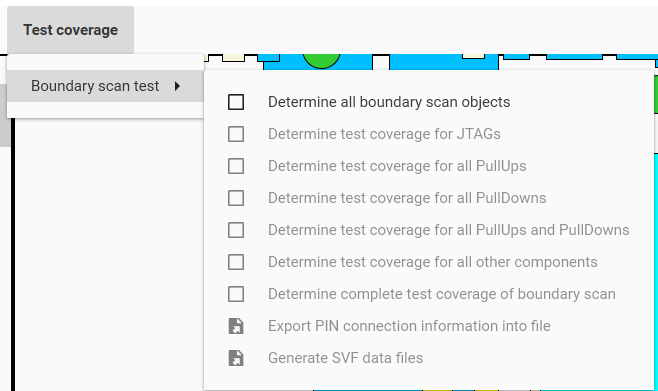
\includegraphics[scale=0.60]{figures/attachments/testCoverage.png}
	\begin{figure}[!h]
	\caption{Test coverage menu group}
	\label{fig:testCoverage}
	\end{figure}
\end{center}

As shown in \ref{fig:testCoverage} within the Test coverage -> Boundary scan test -> menu group there are the following menu items available:
\begin{itemize}
	\item Determine all boundary scan objects - before being able to perform any other test related action you have first to choose this one. (Settings will be considered)
	\item Determine test coverage for \ac{JTAG}s
	\item Determine test coverage for all PullUps
	\item Determine test coverage for all PullDowns
	\item Determine test coverage for all PullUps and PullDowns
	\item Determine test coverage for all other components
	\item Determine complete test coverage of boundary scan
	\item Export PIN connection information into file
	\item Generate \ac{SVF} data files
\end{itemize}

\subsection{Determine all boundary scan objects}
After you selected Test coverage -> Boundary scan test -> Determine all boundary scan objects then the objects list should be filled with new selection possibilities:

\begin{center}
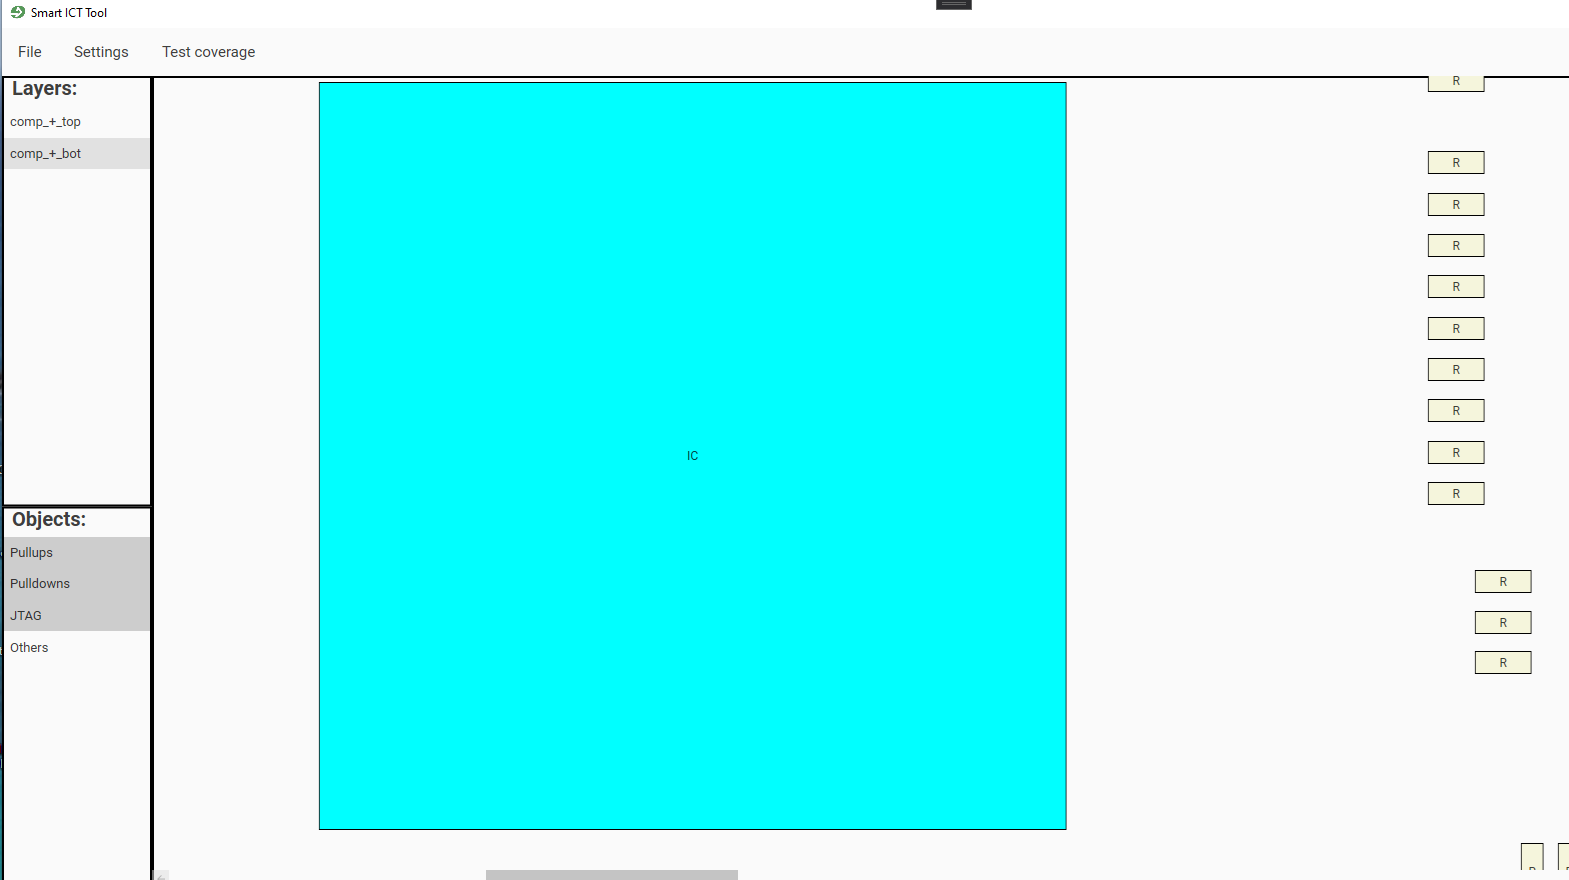
\includegraphics[width=1.00\textwidth]{figures/attachments/dterminedTestCoverageObjects.png}
	\begin{figure}[!h]
	\caption{Determine all boundary scan objects}
	\label{fig:dterminedTestCoverageObjects}
	\end{figure}
\end{center}

Now you could (\ref{fig:dterminedTestCoverageObjects}) select just the test coverage related objects of interest to be shown within the component view.

\subsection{Performing any test coverage of objects}

After you click for example on Test coverage -> Boundary scan test -> Determine test coverage for all PullUps then the calculated value will be shown as text and further more each connection to a according pull up resistor will be shown in green color:

\begin{center}
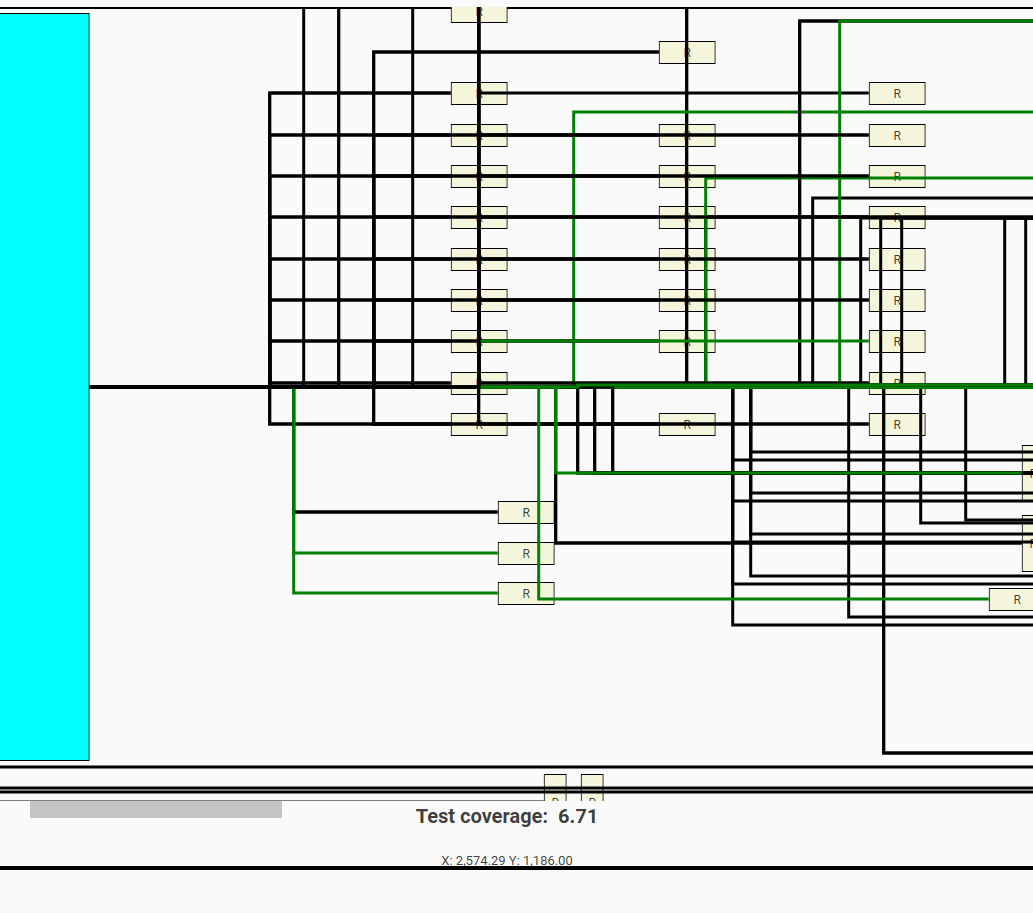
\includegraphics[width=1.00\textwidth]{figures/attachments/pullUpsTEstCoverage.png}
	\begin{figure}[!h]
	\caption{Determine test coverage for all PullUps}
	\label{fig:pullUpsTEstCoverage}
	\end{figure}
\end{center}

If you click again on Test coverage -> Boundary scan test -> Determine test coverage for all PullUps then the according check box will be unchecked and every connection is been showed just in black color again. This kind of procedure is also available for all other operations to detect the test coverage.

\subsection{Export PIN connection information into file}

After you click on Test coverage -> Boundary scan test -> Export PIN connection information into file a new dialog should appear where you can select the destination of file saving. After you selected that then the according file should be generate containing all pin information of interest of all \ac{JTAG} devices of the loaded project.

\subsection{Generate SVF data files}
If you click on Test coverage -> Boundary scan test -> Generate \ac{SVF} data files then first a dialog will be shown to select the target folder where to save the created files at. This folder will only be considered if you are not working in the project file mode. If so the files will be automatically been saved within the project file. Afterward you will be asked for selecting the according \ac{BSDL} file for all \ac{JTAG} devices found. After you selected the \ac{BSDL} file you will be informed about to make sure that the programmer is correctly connected to the \ac{JTAG} device as the default vector first needs to be read out:

\begin{center}
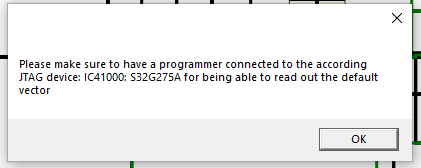
\includegraphics[scale=0.60]{figures/attachments/makeSureToConnect.png}
	\begin{figure}[!h]
	\caption{Make sure to have a programmer connected}
	\label{fig:makeSureToConnect}
	\end{figure}
\end{center}

After you confirmed the dialog \ref{fig:makeSureToConnect} then the read out will be performed and the according \ac{SVF} files for playing the pull down and pull up resistors will be generated.

\section{Log panel}

By clicking on the expander which is located at the very bottom of the application the log panel will be visible. It contains every single message logged during the working with the tool:

\begin{center}
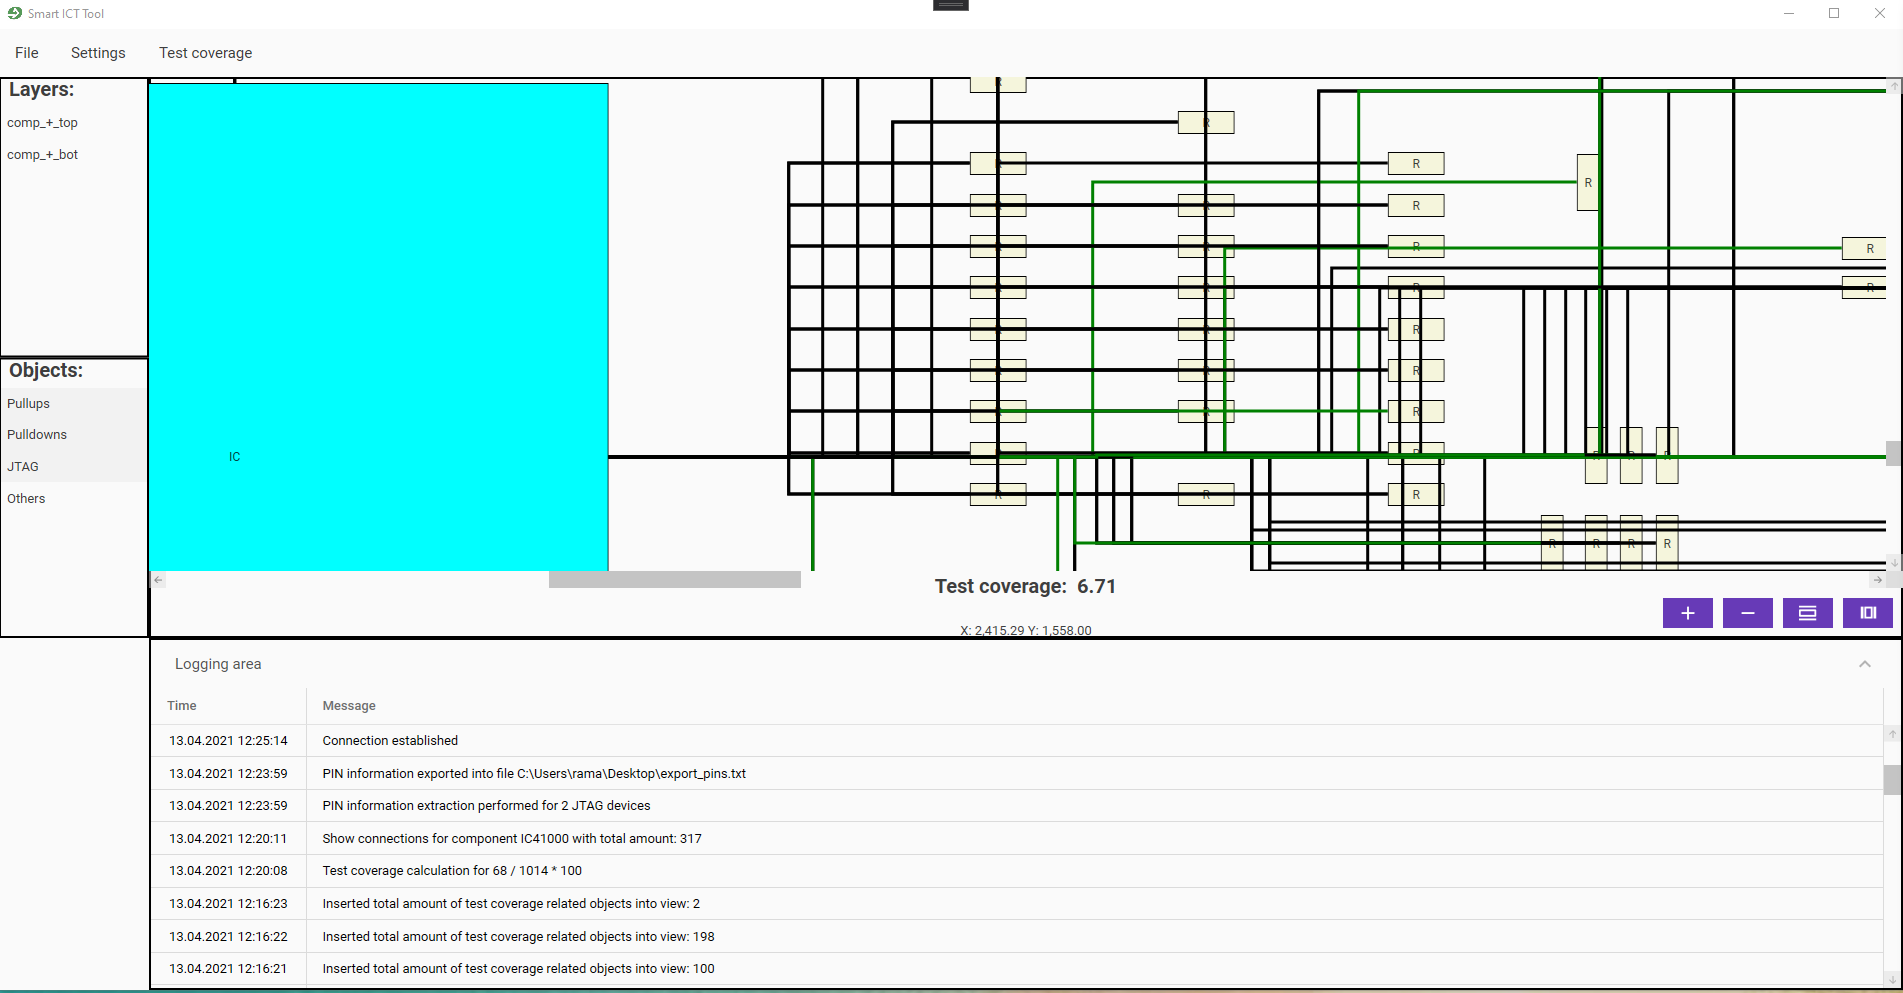
\includegraphics[width=1.00\textwidth]{figures/attachments/logging.png}
	\begin{figure}[!h]
	\caption{Logging area}
	\label{fig:logging}
	\end{figure}
\end{center}

\section{Drag and drop within the application}
You are further able to drag and drop directly files or folders to the application area. If something valid was dropped then it automatically should be opened or imported and if project mode is enabled saved further within the project file